\chapter{The Pigeonhole Principle}
\label{chapter:pigeonhole}
\marginurl{%
  The Pigeonhole Principle:\\\noindent
  Introduction to Combinatorics \#3
}{youtu.be/1D1Fa7WIUO8}

The principle we are going to discuss in this chapter is very simple, it states
that if you have more objects than boxes, then you cannot put all the objects into
boxes without putting two objects into the same box.

More formally the principle can be formulated as follows: if $n > m$, then any
function from $\range{n}$ to $\range{m}$ is not an injection. This simple
statement is famous in mathematics and called 
\emph{the pigeonhole principle}\footnote{%
  The pigeonhole principle is also called the Dirichlet principle, after the
  German mathematician G. Lejeune Dirichlet, who demonstrated, using this
  principle, that there were at least two Parisians with the same number of
  hairs on their heads.
}.

\begin{theorem}[the pigeonhole principle]
  Let $X$ and $Y$ be some sets such that $\cardinality{X} > \cardinality{Y}$.
  Then for any function $f : X \to Y$ there are $x_0 \neq x_1 \in X$ such that
  $f(x_0) = f(x_1)$.
\end{theorem}
\begin{proof}
  The statement follows from
  Theorem~\ref{theorem:injections-surjections-inequalities}.
\end{proof}

This simple statement is very handy in combinatorics. For example, using this
statement one may prove that in any group of more than $12$ people there are
two people who were born in the same month.

Assume that there are $n$ people in the group and $n > 12$.
Consider the following function $f : \range{n} \to \range{12}$ such that $f(i) = j$ if the
$i$th person was born in $j$th month. Note that $f$ is not an injection since
$n > 12$ i.e. there are $i_0 \neq i_1$ such that $i_0$th and $i_1$th person are
born in the same month.

\begin{exercise}
  Show that among any group of five (not necessarily consecutive)
  integers, there are two with the same remainder when divided by $4$.
\end{exercise}

We may also prove that in any group of people there are two people who are
friends with the same number of people in the group.

Assume the number of people is $n$. It is easy to see that every person may
have at most $n - 1$ friends. Hence, we may define a function $f: \range{n} \to
\set{0, \dots, n - 1}$ such that $f(i)$ is equal to the number of friends in
this group of the $i$th person in this group.
We need to consider two cases.
\begin{itemize}
  \item If $\Im f \subseteq \range{n - 1}$, then
    $\cardinality{\range{n}} > \cardinality{\Im f}$ and $f$ is not an injection.
  \item Otherwise, note that it is not possible that $(n - 1) \in \Im f$
    because if there is a friend with no friends it is not possible that there
    is a friend who is friends with everyone. Hence,
    $f : \range{n} \to \set{0, 1, \dots, n - 2}$ and $f$ is not an injection.
\end{itemize}

\begin{theorem}[Erd\H{o}s–-Szekeres]
  Every sequence of $(r - 1)(s - 1) + 1$ distinct real numbers contains a
  subsequence of length $r$ that is increasing or a
  subsequence of length $s$ that is decreasing.
\end{theorem}
\begin{proof}
  Given a sequence of length $(r - 1)(s - 1) + 1$, label each number $x_i$ in
  the sequence with the pair $(a_i, b_i)$, where $a_i$ is the length of the
  longest increasing subsequence ending with $x_i$ and $b_i$ is
  the length of the longest decreasing subsequence ending with $x_i$.
  Each two numbers in the sequence are labeled with a different pair: if $i < j$
  and $x_i < x_j$ then $a_i < a_j$, and on the other hand if $x_i > x_j$ then
  $b_i < b_j$. But there are only $(r - 1)(s - 1)$ possible labels if $a_i$ is
  at most $r - 1$ and $b_i$ is at most $s - 1$, so by the pigeonhole principle
  there must exist a value of $i$ for which $a_i$ or $bi$ is outside this
  range. If $a_i$ is out of range then $x_i$ is part of an increasing sequence of
  length at least $r$, and if $b_i$ is out of range then $x_i$ is part of a
  decreasing sequence of length at least $s$.
\end{proof}

We can also use the pigeonhole principle to show that the lower bound from
\Cref{theorem:guess-one-out-of-many} is precise.
\begin{theorem}
  There is a $B$-decision tree $T$ such that $h(T) \le 9$ and 
  $\mathrm{val}(T, S) \in S$ for all $S \in \binom{\range{1000}}{500}$.
\end{theorem}
\begin{proof}
  Let us fix some set $S \in \binom{\range{1000}}{500}$. Note that $S \cap
  \range{501} \neq \emptyset$. Therefore, the minimal element of $S$ belongs to
  $\range{501}$. Hence, using an algorithm similar to the algorithm from
  \Cref{chapter:structural-induciton}, we can find the minimal element of $S$
  using at most $\ceil{\log{501}} = 9$ questions.
\end{proof}
\nomenclature[U]{$\ceil{\alpha}$}{denotes the smallest integer greater than or
equal to $\alpha$}

\section{The Generalized Pigeonhole Principle}
One may generalize the pigeonhole principle in the following way.
If $N$ objects are placed into $k$ boxes, then there is at least one box
containing at least $\ceil{N / k}$ objects.
\begin{theorem}[the generalized pigeonhole principle]
\label{theorem:generalized-pigeonhole-principle}
  Let $X$ and $Y$ be some sets. Then for any function $f : \cardinality{X} \to
  \cardinality{Y}$ there are $x_1, \dots, x_\ell \in X$ such that
  \begin{itemize}
    \item $f(x_i) = f(x_j)$,
    \item $x_i \neq x_j$ for any $i \neq j \in \range{\ell}$, and
    \item $\ell \ge \ceil{\cardinality{X} / \cardinality{Y}}$, where
      $\ceil{\alpha}$ denotes the least integer greater than or equal to
      $\alpha$.
  \end{itemize}
\end{theorem}

Now we illustrate applications of this principle on some examples and prove the
statement in the next section.

Using this theorem we can prove that if we draw $9$ cards out of a deck of
cards, we are guaranteed that at least three of them are of the same suit.
Given that, there are $4$ suits in the deck, by pigeonhole principle if we put each card into
one of the four boxes according to their suits, one of the boxes should have
at least $\ceil{9 / 4} = 3$ cards.

Another example shows how the generalized pigeonhole principle can be applied
to an important part of combinatorics called Ramsey theory.

Assume that in a group of six people, each pair of individuals consists of two
friends or two enemies. One may prove that there are either three mutual
friends or three mutual enemies in the group.

Let $A$ be one of the six people; of the five other people in the group, there
are either three or more who are friends of $A$, or three or more who are
his enemies $A$. This statements follows from the generalized pigeonhole
principle since when five objects are divided into two sets, one of the sets
has at least $\ceil{5 / 2} = 3$ elements. Without loss of generality we may
suppose that $B$, $C$, and $D$ are friends of $A$. If any two of these three
individuals are friends, then these two and $A$ form a group of three mutual
friends. Otherwise, $B$, $C$, and $D$ form a set of three mutual enemies.

\section{The Averaging Principle}
Assume that we have a collection of $m$ objects, the $i$th of which has
``size'' $l_i$. We wish to show that at least one of the objects is large.
In this situation we can argue that at least one of the objects has size
greater or equal to the average size ($\sum l_i / m$).
\begin{theorem}[the averaging principle]
\label{theorem:averaging-principle}
  Every sequence of numbers has a number at least as large as the average and a
  number at least as small as the average; i.e. for any sequence $a_1$, \dots,
  $a_m$ there are $i$ and $j$ such that
  \begin{gather*}
    a_i \ge \frac{1}{m} \sum_{i = 1}^m a_i \\
    \text{and} \\
    a_j \le \frac{1}{m} \sum_{i = 1}^m a_i.
  \end{gather*}
\end{theorem}
\begin{proof}
  We prove only the existence of $i$, proof of the existence of $j$ is almost
  the same.

  Assume the opposite, i.e. that $a_i < \sum_{i = 1}^n a_i / m$
  for any $i \in \range{n}$. Note that this implies that
  $\sum_{i = 1}^n a_i \le m \cdot \sum_{i = 1}^n a_i / m = \sum_{i = 1}^n a_i$.
  Which is a contradiction.
\end{proof}

\begin{exercise}
  Finish the proof of Theorem~\ref{theorem:averaging-principle}
\end{exercise}

Like the pigeonhole principle, this principle is very simple but the
applications of it are surprisingly interesting.

First, it allows to prove the generalized pigeonhole principle.
\begin{proof}[Proof of Theorem~\ref{theorem:generalized-pigeonhole-principle}]
  Let $Y = \range{m}$ (it is easy to see that the proof works for any other finite
  $Y$). Define the sequence $a_i = \cardinality{f^{-1}(i)}$.
  Note that we need to prove that $a_i \ge \ceil{\cardinality{X} / m}$ for some
  $i \in \range{m}$

  It is clear that $\bigcup_{i = 1}^m f^{-1}(i) = X$ and that $f^{-1}(i) \cap
  f^{-1}(j) = \emptyset$ for any $i \neq j \in \range{m}$. Thus, by the additive
  principle, $\sum_{i = 1}^m a_i = \cardinality{X}$. Hence, by the averaging
  principle, $a_i \ge \cardinality{X} / m$ for some $i \in \range{m}$. However,
  $a_i$ is an integer, thus $a_i \ge \ceil{\cardinality{X} / m}$.
\end{proof}

Another nice application of the averaging principle allows us to prove that if
in some group (with more than one person) the number of pairs of people who
know each other is less than $n - 1$, then we can split this group into two
subgroups such that people from different subgroups do not know each other.

Let us assume that there are $n$ people in the group. We prove the statement
using the induction by $n$.
\begin{description}
  \item [(the base case)] If $n = 2$, there are less than $n - 1 = 1$ pairs
    of people who know each other, in other words, these two people in the
    group do not know each other. Thus we can put each of them into a separate
    subgroup.
  \item [(the induction step)] Let $p_i$ ($i \in \range{n}$) be the number of
    acquaintances of the $i$th person. Note that
    $\sum_{i = 1}^n p_i \le 2(n - 2)$ since we count each pair twice.
    By the averaging principle, $p_i \le 2(n - 2) / n = 2 - 2 / n$ for some
    $i \in \range{n}$.  Thus $p_i$ is either $0$ or $1$.
    \begin{itemize}
      \item If $p_i = 0$, we can put the $i$th person into the first subgroup
        and everyone else into another.
      \item If $p_i = 1$ we consider the group of $n - 1$ people without the
        $i$th person, by the induction hypothesis, we can split everyone but
        $i$th person into two subgroups and since the $i$th person has only one
        acquaintance we can put them in the same subgroup.
      \end{itemize}
\end{description}



\begin{chapterendexercises}
  \exercise Let $ABC$ be an equilateral triangle such that the length of $AB$ is
    equal to $1$, and let $p_1$, \dots, $p_5$ be points inside of $ABC$.
    Show that there are $i \neq j \in \range{5}$ such that the distance between 
    $p_i$ and $p_j$ is at most $0.5$.
  \exercise We are given $17$ points inside a regular triangle of side of
    length $1$. Prove that two of these points have distance at most $1 / 4$.
    \begin{solution}
      In order to do it let us consider the following partition of the triangle.

      \begin{center}
        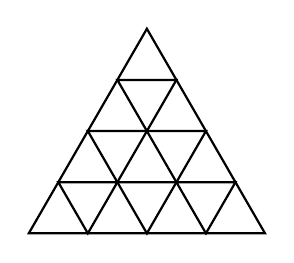
\begin{tikzpicture}[thick, scale=0.3]
          \draw (-5,0) 
            -- (5,0)
            -- (0, 8.660) 
            -- cycle;
          \draw (0,0) 
            -- (-2.5,4.330)
            -- (2.5,4.330)
            -- cycle;
          \draw (-2.5,0) 
             -- (-3.75,2.165)
             -- (-1.25,2.165)
             -- cycle;
          \draw (2.5,0) 
             -- (3.75,2.165)
             -- (1.25,2.165)
             -- cycle;
          \draw (0,4.330) 
             -- (-1.25,6.495)
             -- (1.25,6.495)
             -- cycle;
          \draw (0,4.330) 
             -- (-1.25,2.165)
             -- (1.25,2.165)
             -- cycle;
        \end{tikzpicture}
      \end{center}

      Note that there are 16 small triangles inside, hence by pigeonhole
      principle there are at least two points in the same small triangle.
      Additionally, distance between any two points inside the regular triangle
      with side $1 / 4$ is at most $1 / 4$.
    \end{solution}
  \exercise Show that if there are 30 students in a class, then at least
    two have last names that begin with the same letter.
  \exercise[recommended] Let $n$ be a positive integer. Show that in any set of
    $n$ consecutive integers there is exactly one divisible by $n$.
    \begin{solution}
      Let the numbers be $k$, $k + 1$, \dots, $k + n - 1$. Assume that all the
      numbers are not divisible by $n$. Consider the function 
      $f: \set{k, k + 1, \dots, k + n - 1} \to \set{1, \dots, n - 1}$ such that
      $f(k + i) \equiv k + i \pmod{n}$. Note that the set on the left has more
      elements than the set on the right, so there are $i_1 < i_2$ such that 
      $k + i_1$ has the same reminder as $k + i_2$.
      Thus $n$ divides $0 < i_2 - i_1 < n$, which is a contradiction.
    \end{solution}
  \exercise[recommended] Prove that for every sequence of integers $a_1$, \dots,
    $a_n$ there are $k > 0$ and $\ell \ge 0$ such that $k + \ell \le n$ and
    $\sum_{i = k}^{k + \ell} a_i$ is divisible by $n$.
    \begin{solution}
      We consider the $n$ sums modulo $n$ of the form $a_1$, $a_1 + a_2$,
      \dots, $a_1 + a_2 + \dots + a_n$. First, we note that if any of these sums
      $a_1 + \cdots + a_\ell \equiv 0 \pmod{n}$, then we are done by picking $k
      = 1$ and $\ell$ accordingly since being equivalent to $0$ modulo $n$ is
      the same as being divisible by $n$. As a result, it suffices to show the
      result when none of the sums are equivalent to $0$ modulo $n$.

      In this case, each of these sums modulo $n$ necessarily must be one of
      $1$, $2$, \dots, $(n - 1)$. That is, there are $n - 1$ possible values for
      each of these $n$ sums. Therefore, by the pigeonhole principle, we must
      have that two of these sums are equivalent modulo $n$. Thus there exists
      $m > 0 $ and $j > 0$ (and without loss of generality may assume that $j >
      m$ ) so that 
      \[
        a_1 + a_2 + \dots + a_m \equiv a_1 + a_2 + \cdots + a_j \pmod{n}.
      \]
      Note that subtracting $ a_1 + a_2 + \cdots + a_m$ from both sides yields
      that 
      \[
        0 \equiv
        a_{m + 1} + \cdots + a_{j} \pmod{n},
      \]
      and hence by taking $k = m + 1$ and $\ell = j - m - 1 = j - k $ we prove that 
      \[
        0 \equiv a_k + a_{k + 1} + \dots + a_{k + \ell} \pmod{n};
      \] 
      in other words, $\sum\limits_{i = 0}^\ell a_{k + i}$ is divisible by $n$.
    \end{solution}
  \exercise[recommended] Let $S \subseteq \range{20}$ be a set. Show that if
    $\cardinality{S} \ge 13$, then there are $a, b \in S$ such that $a - b = 6$.
  \exercise Let $S \subseteq \range{20}$ be a set. Show that if $\cardinality{S}
    \ge 11$, then there are $a \neq b \in S$ such that $a + b = 21$.
    \begin{solution}
      Note that there are $10$ pairs $(1, 20)$, \dots, $(10, 11)$ such that their
      sum is equal to $21$. Hence, by the pigeonhole principle, there are two
      elements of $S$ such that they belong to the same pair; i.e. their sum is
      equal to $21$.
    \end{solution}
  \exercise How many numbers must be selected from the set $\range{6}$ to
    guarantee that at least one pair of these numbers add up to $7$?
  \exercise Sasha is training for a triathlon. Over a $30$ day period, he
    pledges to train at least once per day, and $45$ times in all. Then there
    will be a period of consecutive days where he trains exactly $14$ times.
  \exercise Show that among any $n + 1$ positive integers not exceeding $2n$
    there must be an integer that divides one of the other integers.
    \hint{Consider the set of holes equal to the set of odd numbers
    from $1$ to $2n$.}
  \exercise Let $A_1, \dots, A_\ell \subseteq \range{n}$ be some sets such that
    $A_i \cap A_j \neq \emptyset$. Show that $\ell \le 2^{n - 1}$.
    \begin{solution}
      We are going to prove this statement using the pigeonhole principle. The
      main component of the proof is the fact that $A \cap \bar{A} = \emptyset$
      for any set $A \subseteq \range{n}$, where $\bar{A} = \range{n} \setminus A$.

      Let $L = \{A_1, \dots, A_\ell\}$ and
      $R = \set[A \subseteq \range{n}]{\set{A, \bar{A}}}$. It is easy to see
      that $\cardinality{R} = 2^{n - 1}$. Define the function $f : L \to R$ such that 
      $f(A_i) = \set{A_i, \bar{A_i}}$. Let us prove that $f$ is an injection; 
      assume the opposite i.e. that there are $i \neq j$ such that 
      $f(A_i) = f(A_j)$. Since $f(A_i) = f(A_j)$ it implies that $A_i =
      \bar{A_j}$ but it contradicts to the statement that $A_i \cap A_j =
      \bar{A_j} \cap A_j = \emptyset$.

      Hence, there is an injection from $L$ to $R$ which implies that
      $\cardinality{L} \le \cardinality{R}$.
      As a result, we proved that $\ell \le 2^{n - 1}$.
    \end{solution}
  \exercise[recommended] Let $a_1$, $a_2$, \dots, $a_t$ be positive integers. Show that
    if $a_1 + a_2 + \dots + a_t - t + 1$ objects are placed into $t$ boxes,
    then for some $i \in \range{t}$, the $i$th box contains at least $a_i$ objects.
    \hint{It is important in this question that $a_1$, \dots, $a_t$ are
    integers.}
  \exercise Let $\set{(x_1,y_1), \dots, (x_5, y_5)} \subseteq \Z^2$ be a
    set of five distinct points with integer coordinates in the xy plane. Show
    that the midpoint of the line joining at least one pair of these points has
    integer coordinates.
  \exercise Let $S \subseteq \range{2n}$ be a set such that 
    $\cardinality{S} = n + 1$. Show
    that there are $x \neq y \in S$ such that $x$ and $y$ are coprime.
  \exercise[recommended] In some school there are three clubs. For each two
    students there is a club such that these students are  members of this club.
    Show that there is a club that at least $2 / 3$ of all students are members
    of this club.
  \exercise Show that the set $\set{7, 77, 777, \dots}$ contains a number
    divisible by $2019$.
  \exercise What is the maximal number of chess knights one may put on a
    chessboard so that they would not attack each other?
  \exercise[recommended] Let us assume that we are given $\ell$ lines that are
    not parallel to each other. Prove that there are at least two of them such
    that angle between them is at most $\pi / \ell$.
    \begin{solution}
      Proof of this statement is very similar to the proof of the averaging
      principle.
      Let us move all the lines (using parallel shift) such that all of them are
      going through $(0, 0)$. Let us denote angles between lines (in clockwise
      order) $\alpha_1$, \dots, $\alpha_{2\ell}$ respectively and assume that
      all of them are greater than $\pi / \ell$. In this case we may note that
      $\sum\limits_{i = 1}^{2\ell} \alpha_i > 2\ell \cdot \pi / \ell = 2\pi$,
      but we know that $\sum\limits_{i = 1}^{2\ell} \alpha_i  = 2\pi$.
    \end{solution}
\end{chapterendexercises}
